\documentclass[11pt,a4paper]{article}

\usepackage[T1]{fontenc}
\usepackage[utf8]{inputenc}
\usepackage[polish]{babel}
\usepackage{lmodern}
\usepackage[margin=2.3cm]{geometry}
\usepackage{graphicx}
\usepackage{amsmath,amssymb}
\usepackage{booktabs}
\usepackage{array}
\usepackage{caption}
\usepackage{float}
\usepackage{enumitem}
\usepackage{fancyhdr}
\usepackage{xcolor}
\usepackage[colorlinks=true,linkcolor=black,urlcolor=blue]{hyperref}

\graphicspath{{src/}}

\captionsetup{font=small,labelfont=bf}
\setlist{itemsep=2pt,parsep=0pt,topsep=3pt}
\renewcommand{\arraystretch}{1.15}

\pagestyle{fancy}
\fancyhf{}
\lhead{\textbf{OPUS 29} - raport}
\rhead{{Paweł Jarosz}}
\rfoot{Strona \thepage}

\begin{document}

\section{Wstęp}

Pełny model przestrzenny guza to równanie różniczkowe cząstkowe na siatce
trójwymiarowej. Takie założenia opisują rozwój dokładne, lecz jego rozwiązanie jest zbyt wolne do interaktywnego planowania terapii.
Można je zredukować do układu dwóch równań zwyczajnych opisujących wyłącznie
całkowitą masę guza $y(t)$, lecz redukcja gubi informację o tym,
gdzie guz się znajduje i gdzie trafiła dawka. Badany pomysł (PI-NODE) polega na zachowaniu mechanistycznego rdzenia ODE i dołożeniu
do niego uczonego członu domykającego, który ma odtworzyć utraconą informację. Jeden przebieg modelu przestrzennego to
2,3~s na GPU (siatka $160^3$, 5,3~mln liczb stanu). Model zredukowany to
6,4~ms na jednym rdzeniu CPU. Jest to około 350$\times$ szybciej, przy stanie złożonym z dwóch liczb. To jest powód, dla którego w ogóle godzimy się na utratę informacji przestrzennej oraz użycie uproszczonego modelu. W dalej części opisze uzyskane wyniki.

\section{Dane referencyjne: GliODIL rozszerzony o radioterapię}

Do wygenerowania prawdziwych przebiegów rozwoju guza skorzystałem z frameworku GliODIL. GliODIL dostarcza dla każdego pacjenta mapy istoty białej i szarej oraz segmentację
guza (BraTS). Na tej podstawie odtwarzamy ciągłą gęstość komórek $A_0(x)$ metodą
dwóch progów. Model bazowy to równanie reakcyjno-dyfuzyjne Fishera--Kołmogorowa:
\begin{equation}
\frac{\partial A}{\partial t} \;=\; \nabla\!\cdot\!\big(D(x)\nabla A\big) + f\,A(1-A),
\qquad
D(x) = \begin{cases} D_w & \text{istota biała}\\[1mm] D_w/r & \text{istota szara},\end{cases}.
\end{equation}
Radioterapię została dołożona na potrzeby naszej symulacji, orginalny framework jej nie uwzględniał. Jest ona opisana przez jedno nowe pole i dwa nowe człony:
\begin{align}
\frac{\partial Z}{\partial t} &= -\frac{Z}{\tau} + U(t)B(x) \label{eq:radiotherapy1} \\
\frac{\partial A}{\partial t} &= \nabla\cdot\big(D\nabla A\big) + fA(1-A) - \gamma(1-hA)ZA \label{eq:radiotherapy2}
\end{align}
Człon $Z$ opisuje naprawialne uszkodzenie, natomiast $A$ opisuje zabijanie komórek. Zmienne w równaniach \eqref{eq:radiotherapy1} i \eqref{eq:radiotherapy2} opsuje tabelka \ref{table:radiotherapy}.

\begin{table}[H]
\centering\small
\begin{tabular}{@{}ll@{}}
\toprule
\textbf{Symbol} & \textbf{Opis} \\
\midrule
$B(x)$      & przestrzenny rozkład dawki (0--1); wygładzony wskaźnik maski celu poszerzonej\\
            & o margines kliniczny, krawędź sigmoidalna modeluje półcień (4~mm)\\
$U(t)$      & przebieg czasowy dawki, impulsy trapezowe, dwie frakcje w $t=15$ i $t=45$\\
$\gamma$    & promieniowrażliwość (losowana na pacjenta)\\
$\tau$      & czas relaksacji / naprawy uszkodzeń\\
$h$         & promieniooporność hipoksyjna, czynnik $(1-hA)$ tłumi zabijanie\\
            & w gęstym, niedotlenionym rdzeniu guza\\
\bottomrule
\end{tabular}
\caption{Wielkości wprowadzone przez rozszerzenie modelu o radioterapię.}
\label{table:radiotherapy}
\end{table}

Tempo wzrostu kalibrujemy dla każdego pacjenta osobno, korzystając z niezmienniczości
Fishera--Kołmogorowa względem przeskalowania czasu ($A(x,ct)$ rozwiązuje układ dla
$(cD, cf)$), tak aby końcowa masa guza odpowiadała rozmiarowi jego własnego guza.

\subsection{Rozważane geometrie promieniowania}

To jest sedno eksperymentu. Obie konfiguracje dostarczają tę samą dawkę w tym samym
harmonogramie i różnią się wyłącznie tym, do jakiej maski anatomicznej dopasowany
jest obszar napromieniany. Model zredukowany widzi dla obu
niemal identyczne $U(t)$, więc różnicy w wyniku z definicji nie da się
odtworzyć bez członu domykającego.

\begin{table}[H]
\centering\small
\begin{tabular}{@{}llcc@{}}
\toprule
\textbf{Konfiguracja} & \textbf{Maska celu} & \textbf{Margines} & \textbf{Pokrycie} \\
\midrule
\texttt{full\_cover}      & obszar FLAIR       & 15 mm & 0,90 \\
\texttt{narrow\_centered} & rdzeń wzmacniający & 5 mm  & 0,42 \\
\bottomrule
\end{tabular}
\caption{Geometrie wiązki. Pokrycie = mediana udziału masy guza znajdującej się
wewnątrz wiązki w chwili $t=0$.}
\end{table}

Rozkład \emph{full cover} to standardowy plan kliniczny dla glejaka: obszar napromieniany
obejmuje całą nieprawidłowość widoczną w sekwencji FLAIR z marginesem 15~mm.
\emph{narrow centered} dopasowuje się natomiast wyłącznie do rdzenia wzmacniającego
się po kontraście, przez co nie obejmuje nacieku rozciągającego się poza nim. Na Rysunku \ref{fig:radiotherapy1} widzimy różnice rozwoju guza nieleczonego oraz poddanego terapii przy użuciu obu rozkładów dawki. Rusunek \ref{fig:radiotherapy2} wizualizuję gęstość komórek guza oraz maskę prominiowania. Rysunek \ref{fig:radiotherapy3} ukazuje stan końcowy dla guza nieleczonego i poddanego każdej z dwóch terapii. Możemy zauważyć, że rozkład \texttt{narrow\_centered} zgodnie z przewidywaniami nie był w stanie zredukować nacieków, przez co guz rozrósł się poza centrum. 

\begin{figure}[H]
\centering
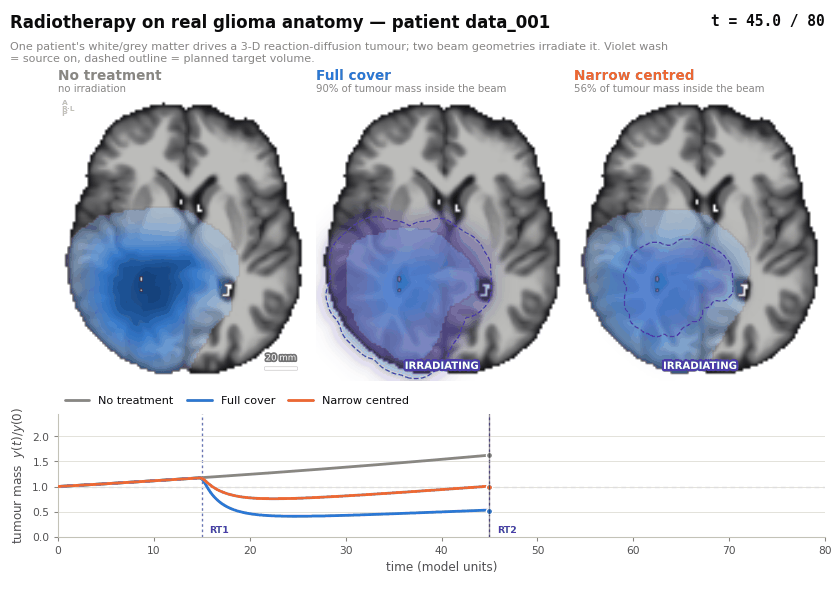
\includegraphics[width=0.93\linewidth]{rys1-geometrie-wiazki.png}
\caption{Moment drugiego napromieniania ($t=45$) u jednego pacjenta. Kolor niebieski oznacza
gęstość komórek nowotworowych, fioletowa poświata wskazuje natężenie radiacji, a kontur przerywany określa
planowany obszar napromieniany. Widać różnicę geometrii: \emph{Full cover} obejmuje cały
guz wraz z naciekiem, \emph{Narrow centred} mieści się w jego wnętrzu i omija naciek. Panel lewy to przebieg bez leczenia. Wykres dolny pokazuje rozchodzenie
się krzywych opisujących masy guza.}
\label{fig:radiotherapy1}
\end{figure}

\begin{figure}[H]
\centering
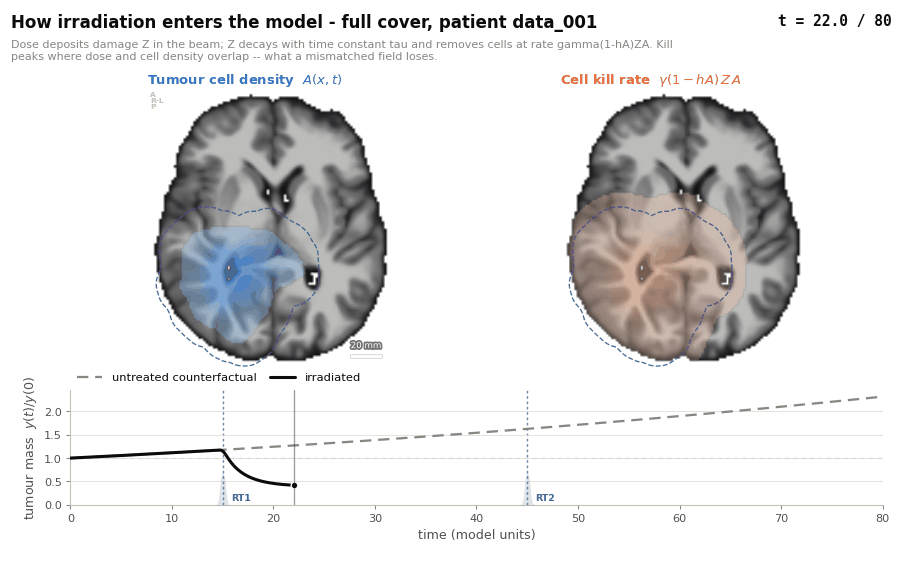
\includegraphics[width=0.93\linewidth]{rys2-mechanizm-dawki.png}
\caption{Mechanizm działania dawki. Po lewej gęstość komórek $A$, po prawej tempo
zabijania $\gamma(1-hA)ZA$. Komórki giną wyłącznie tam, gdzie dawka i gęstość
komórek nakładają się na siebie.}
\label{fig:radiotherapy2}
\end{figure}

\begin{figure}[H]
\centering
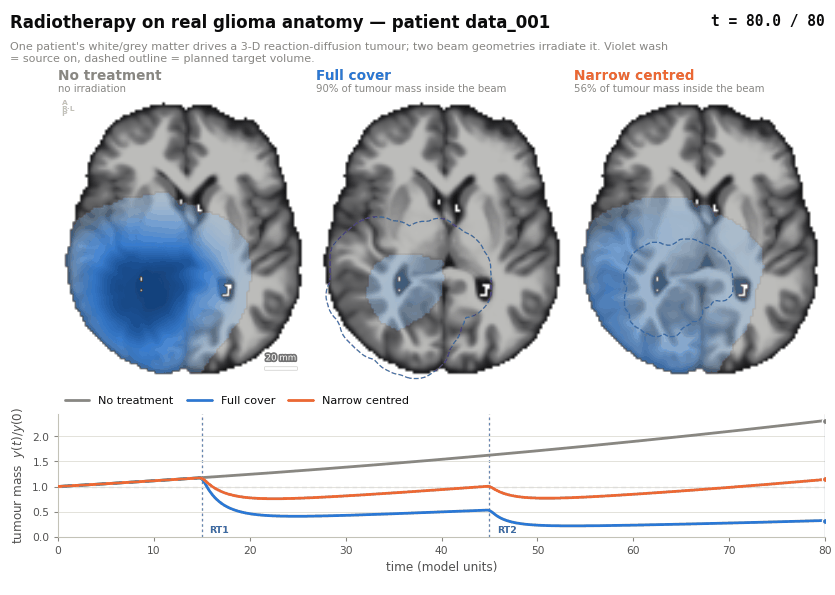
\includegraphics[width=0.93\linewidth]{rys3-wynik-koncowy.png}
\caption{Stan końcowy. Bez leczenia guz rośnie do 2,3$\times$ masy początkowej, przy
pełnym pokryciu spada do 0,32$\times$, natomiast przy wąskiej wiązce \emph{odrasta} do
1,14$\times$, czyli powyżej stanu wyjściowego. W przekrojach widać pozostałość guza:
przy \emph{full cover} prawie nic nie zostało, przy \emph{narrow centred} przetrwał
cały naciek poza rdzeniem.}
\label{fig:radiotherapy3}
\end{figure}

\section{Dane treningowe}

Dla każdego z 117 pacjentów generujemy trzy trajektorie referencyjne: przebieg bez
leczenia oraz po jednej dla każdej z dwóch geometrii wiązki. Każda z nich to pełna
symulacja trójwymiarowa na siatce $160^3$ (woksel 1,5~mm), całkowana przez $T=80$
jednostek czasu krokiem $\Delta t = 0{,}1$, czyli 800 kroków na przebieg. Z tych
trajektorii odczytujemy całkowitą masę guza $y(t)$, która jest jedyną wielkością
widzianą później przez modele zastępcze. W tabelce \ref{tab:train} przedstawione zostały parametry  wygenerowanych danych treningowych. Przeliczenie przebiegów uczących trwało około 60min na czterech kartach Ada 6000 48GB VRAM.

\begin{table}[H]
\centering\small
\begin{tabular}{@{}p{3.1cm}p{12.2cm}@{}}
\toprule
\textbf{Obserwacje} & 20 próbek $y(t)$ w oknie $t \in [14,35]$ (obejmuje całą pierwszą frakcję)\\
\textbf{Szum} & $\mathcal{N}\big(0,(0{,}02\,y_i)^2\big)$, 20 niezależnych realizacji\\
\textbf{Okno prognozy} & $(35,80]$: zawiera drugie, niewidziane napromienianie\\
\textbf{Skala} & 117 pacjentów $\times$ 2 konfiguracje = 234 kolumny $\times$ 20 realizacji
szumu = 4\,680 niezależnie dopasowanych modeli na metodę\\
\bottomrule
\end{tabular}
\caption{Protokół dopasowania, wspólny dla wszystkich porównywanych modeli.}
\label{tab:train}
\end{table}

\section{Modele}

Porównałem ze sobą trzy modele na dokładnie korzystając z tej samej procedury uczącej, tak aby
różnice wynikały z modelu. Wszystkie trzy przewidują tę
samą wielkość, całkowitą masę guza $y(t)=\int_\Omega A\,dx$, i wszystkie dostają ten
sam znany przebieg dawki $U(t)$.

\subsection{ODE}
\label{sec:model-ode}

Punktem wyjścia jest scałkowanie równania przestrzennego po całej dziedzinie. Człon
dyfuzyjny znika (brak przepływu przez brzeg), więc
\begin{equation}
\dot y \;=\; \underbrace{\int_\Omega \nabla\!\cdot\!(D\nabla A)\,dx}_{=\,0}
\;+\; f\!\int_\Omega A\,dx \;-\; f\!\int_\Omega A^2\,dx
\;-\; \gamma\!\int_\Omega (1-hA)\,Z\,A\,dx .
\label{eq:redukcja}
\end{equation}
Pierwsza całka daje $f y$, ale dwie pozostałe nie domykają się: zależą od
rozkładu $A$ i $Z$, a nie tylko od ich całek. Model zredukowany musi je czymś
zastąpić. Ten krok jest źródłem całego błędu strukturalnego:
\begin{equation}
\int_\Omega A^2\,dx \;\approx\; \frac{y^2}{K},
\qquad
\int_\Omega (1-hA)\,Z\,A\,dx \;\approx\; z\,y ,
\end{equation}
gdzie $z(t)$ to skalarny zamiennik pola radiacji. Podstawienie daje klasyczną postać
logistyczną z członem zabijania proporcjonalnym do $z y$.

\paragraph{Poprawka wykładnika.} Człon $f y$ zakłada, że \emph{każda} komórka się dzieli.
W równaniu Fishera--Kołmogorowa proliferacja zachodzi jednak głównie na froncie, który
porusza się ze stałą prędkością $c = 2\sqrt{Df}$. Zatem jego objętość rośnie zgodnie z równaniem
$(a+ct)^3$, czyli $y \sim (a+ct)^3$, skąd
\begin{equation}
\dot y \;=\; 3c\,(a+ct)^2 \;=\; 3c\,y^{2/3}
\qquad\Longrightarrow\qquad
\dot y \;\propto\; y^{2/3},
\end{equation}
a nie $\dot y \propto y$. Dlatego dopuszczamy ogólny wykładnik $q$, przyjmując
$q=1$ (logistyczny), $q=2/3$ (objętościowy, zgodny z powyższym) albo
$q$ uczony z danych. Ostateczny model to układ dwustanowy:
\begin{equation}
\boxed{\;
\dot y = \rho\,y^{q}\Big(1-\frac{y}{K}\Big) - \gamma\,z\,y - \mu\,y ,
\qquad
\dot z = -\frac{z}{\tau} + U(t) \; }
\label{eq:ode}
\end{equation}
z parametrami $\theta=(\rho,K,\gamma,\mu,\tau,q)$, gdzie $\rho$ to tempo proliferacji,
$K$ pojemność środowiska, $\gamma$ promieniowrażliwość stanu zredukowanego, $\mu$ stałe
ubytki, a $\tau$ czas naprawy uszkodzeń. Wszystkie dodatnie dzięki
transformacie softplus z progami.

\subsection{NODE}
\label{sec:model-node}

Drugie skrajne podejście rezygnuje z domykania \eqref{eq:redukcja} wzorem i korzysta jedynie z sieci neuronowej do przewidywania wartości $\dot{y}$:
\begin{equation}
\dot y = g_1(y,z,t,U) \;-\; \mathrm{softplus}\Big(g_2\big(y,z,t,U\big)\Big)\,z\,y ,
\qquad
\dot z = \alpha\,U(t) - \frac{z}{\tau}.
\label{eq:node}
\end{equation}
Dwa wyjścia sieci pełnią różne role: 
\begin{itemize}
    \item $g_1$ -- swobodny człon wzrostu.
    \item $g_2$ -- składnik przewidujący zabijanie komórek. Dzięki przepuszczeniu przez softplus, zagwarantowane są wartości dodatnie, oraz przemnożenie przez $z$ oraz $y$ grarantuje propocjonalność do skumulowanego promieniowania oraz liczby komórek.
\end{itemize}
Ten model nie jest w pełni bezstrukturalny, bo zatrzymuje równanie na
$z$ oraz dwuliniową postać członu radiacji. Dla tego równiania przepada
interpretowalna parametryzacja wzrostu: $\rho$, $K$ i $q$ znikają wewnątrz wag sieci.

\subsection{PI-NODE}
\label{sec:model-pinode}

Jest to model hybrydowy, dodający do równania \eqref{eq:ode} uczoną sieć neuronową, która koryguję błedy wprowadzone przez całkowanie \eqref{eq:redukcja}.  Model ten jest opisany równaniem:

\begin{equation}
\dot y \;=\; \omega\underbrace{\, f_{\mathrm{RT}}(y,z,U;\theta)}_{\text{fizyka}}
\;+\; s_r\underbrace{\, g_{\psi}(y,z,t,U)}_{\text{sieć neuronowa}},
\qquad
\dot z \;=\; -\frac{z}{\tau} + U(t),
\label{eq:pinode}
\end{equation}
gdzie $f_{\mathrm{RT}}$ jest dokładnie prawą stroną
z ~\eqref{eq:ode}, natomiast człon $g_\psi$ to sieć dwuwarstwowa (32 neurony na warstwę, ReLU)
o wejściu $(y,\,z,\,t/T,\,U)$ i jednym wyjściu. Dwie cechy implementacji są istotne dla interpretacji wyników. Po pierwsze, sieć neuronowa $g_\psi$ startuje wyzerowana, więc w chwili startu $g_\psi \equiv 0$ i model jest
dokładnie modelem ODE. Po drugie, $g_\psi$ nie jest niczym ograniczony co do amplitudy. Jedyne, co
ogranicza jego wpływ, to mnożnik $s_r$. To właśnie dlatego $s_r$ okazuje się decydować
o dokładności (rozdz.~\ref{sec:cechowanie}), a różnica między PI-NODE a NODE
z \eqref{eq:node} polega nie tyle na obecności fizyki, ile na tym, że w PI-NODE swoboda
sieci jest przeskalowana w dół poprzez obecność członu mechanistycznego. 

\section{Trening}
\label{sec:trening}

Wszystkie trzy modele przechodzą identyczną procedurę treningową. Dzięki temu różnicę w wynikach można przypisać konkretnemu modelowi, a nie sposobowi uczenia/dopasowania.

\subsection{Dopasowywane parametry}

Parametry wejściowe to para (pacjent, geometria wiązki) wraz z jedną realizacją
szumu. Dla każdej kolumny dopasowujemy osobny, niezależny komplet parametrów. Zbiory parametrów różnią się między modelami:
\begin{align}
\text{ODE}     &:\quad \Theta = \theta = (\rho, K, \gamma, \mu, \tau)
                  \;\;[\,{+}\,q \text{ dla wariantu uczonego}\,], \\
\text{NODE}    &:\quad \Theta = (\psi_{\mathrm{sieci}}, \alpha, \tau), \\
\text{PI-NODE} &:\quad \Theta = (\psi_{\mathrm{sieci}}, \theta),
\end{align}
przy czym wagi $\omega$ i $s_r$ nie należą do $\Theta$, są ustalane z góry
(rozdz.~\ref{sec:cechowanie} pokazuje, dlaczego próba ich uczenia nie ma sensu).

\subsection{Funkcja straty}

Warunek początkowy nie jest uczony, tylko brany z pierwszej obserwacji:
$y(t_0) = \tilde y_1$, $z(t_0) = 0$. Trajektoria powstaje przez scałkowanie modelu, a
strata mierzy niezgodność z obserwacjami w oknie asymilacji:
\begin{equation}
\mathcal{L}(\Theta) \;=\; \underbrace{\frac{1}{N}\sum_{i=1}^{N}
\big(y_\Theta(t_i) - \tilde y_i\big)^2}_{\text{dopasowanie do danych}}
\;+\; \underbrace{\lambda_{2}\,\big\langle g_\psi^2 \big\rangle}_{\text{regularyzacja członu uczonego}},
\label{eq:strata}
\end{equation}
gdzie $\tilde y_i$ to zaszumiona obserwacja, a $\langle\cdot\rangle$ oznacza średnią po
losowo wybranym bloku punktów trajektorii. Dla modelu ODE drugi składnik
znika (nie ma $g_\psi$). Modele uczone są za pomocą optymizatora Adam przez 1200 epok. Wykorzystywane jest wygaszanie kosinusowe.

\subsection{Jak mierzymy wynik}

Wytrenowany model porównujemy z wynikami z pełnej symulacji modelu przestrzennego. Miarą jest względny błąd RMSE liczony osobno w oknie
asymilacji i w oknie prognozy:
\begin{equation}
\mathrm{relRMSE}(\mathcal{T}) \;=\; 100\,\%\;\cdot\;
\frac{\sqrt{\frac{1}{|\mathcal{T}|}\sum_{t\in\mathcal{T}} \big(y_\Theta(t) - y^{\mathrm{PDE}}(t)\big)^2}}
     {\sqrt{\frac{1}{|\mathcal{T}|}\sum_{t\in\mathcal{T}} y^{\mathrm{PDE}}(t)^2}},
\qquad
\mathcal{T} \in \{\,[14,35],\;(35,80]\,\}.
\label{eq:metryka}
\end{equation}
Normalizacja przez wielkość sygnału czyni błędy porównywalnymi między pacjentami
o różnej masie guza. Okno $(35,80]$ zawiera drugie napromienianie,
którego model nigdy nie widział, dzięki czemu ekspryment pokazuje zdolność modelu do przewidywania kolejnych stanów.

\section{Wyniki}
\label{sec:wyniki}

W Tabelce \ref{tab:dokladnosc} zawarte są wyniki otrzymane przez model. Porównanie zostało przeprowadzone dla modeli ODE z $q=1$, $q=\frac{2}{3}$, modelu NODE oraz modelu PI-NODE z różnymi wartościami parametrów $\omega, s_r$. W pierwszej kolumnie znajduje się mediana RMSE z wszystkich eskperymentów, następnie rozstęp ćwiartkowy IQR. Dwie ostatnie kolumny to wartości RMSE dla rozkładu dawki \emph{full cover} oraz \emph{narrow}.

\begin{table}[H]
\centering\footnotesize
\setlength{\tabcolsep}{6pt}
\begin{tabular}{@{}lrrrrr@{}}
\toprule
\textbf{Model} & \textbf{Mediana} & \textbf{IQR} & \textbf{full cover} & \textbf{narrow} \\
\midrule
ODE ($q=2/3$)          & 29,09 & \textbf{14,4} & 30,5 & 28,5 \\
ODE ($q=1$)      & 30,25 & 19,5 & 38,5 & 27,8 \\
NODE           & 32,52 & 20,8 & 45,6 & 28,3 \\
\midrule
PI-NODE, $(\omega = 0{,}005 ; s_r = 0{,}005)$        & 14,73 & 25,9 & 33,9 & 7,8 \\
\textbf{PI-NODE, $(\omega = 0{,}002; s_r=0{,}002)$} & \textbf{12,76} & 18,0 & \textbf{25,1} & \textbf{7,1} \\
\bottomrule
\end{tabular}
\caption{Względny błąd RMSE prognozy w oknie $(35,80]$.
Wszystko przy tym samym budżecie uczenia (1200 epok), więc wiersze są bezpośrednio
porównywalne.}
\label{tab:dokladnosc}
\end{table}

Patrząc na Tabelę ~\ref{tab:dokladnosc}, możemy sformułować trzy wnioski:

\begin{enumerate}
\item Model hybrydowy wygrywa z oboma modelami. PI-NODE
przy dobrze dobranych wagach daje 12,76\,\% wobec 29,09\,\% dla ODE (sama fizyka) i
32,52\,\% dla NODE (samo uczenie). Oba te modele wypadają niemal identycznie
źle, ale z zupełnie innych powodów, co widać w rozdz.~\ref{sec:pasma}.

\item Tam, gdzie redukcja gubi informację, przewaga PI-NODE jest spora.
Dla geometrii \emph{narrow centered}, w której wiązka nie obejmuje nacieku,
PI-NODE daje 7,1\,\% wobec 28,5\,\% dla modelu mechanistycznego.

\item NODE wypada najgorzej. Mimo, że NODE ma więcej swobody niż PI-NODE wypada nagorzej. W PI-NODE człon uczony jestprzemnożony przez małe $s_r$, które ogranicza jego wpływ. Kontrola skali członu
uczonego jest tu ważniejsza niż obecność równania ODE.
\end{enumerate}

\subsection{Liczba i zaszumienie obserwacji}
\label{sec:pasma}

W kolejnym eksperymentcie sprawdziłem rozrzut modelu wywołany szumem
pomiarowym. Aby to zbadać przeprowadziłem eksperymenty na wybranej trajektorii dla jednego pacjęta.

\begin{enumerate}
\item Bierzemy jedną trajektorię ground truth --- pacjenta będącego \emph{medianą} wszystkich przebiegów dla
danej geometrii, więc obraz jest reprezentatywny.
\item Dla każdej liczby próbek $N \in \{5, 10, 15, 20\}$ w oknie asymilacji losujemy
niezależnych realizacji szumu na poziomie
$\varepsilon_i \sim \mathcal{N}\!\big(0,\,(0{,}05\,y_i)^2\big)$. Odchylenie 5\,\% oznacza,
że przedział $\pm 2\sigma$ obejmuje $\pm 10\,\%$ wartości.
\item Do każdej realizacji dopasowujemy osobno każdy z trzech modeli, co daje 80 niezależnych
prognoz.
\item Rysujemy medianę zespołu oraz pasmo percentyli 25--75.
\end{enumerate}

Pasmo jest więc dokładnie tym rozrzutem prognozy, który wywołuje sam szum pomiarowy. Na Rysunku \ref{fig:pasma-waska} zobaczyć możemy dopasowanie poszczególych modeli, natomiast Tabelka \ref{tab:pasma} zawiera faktyczne wartości opisujące dopasowanie modeli.

\begin{figure}[H]
\centering
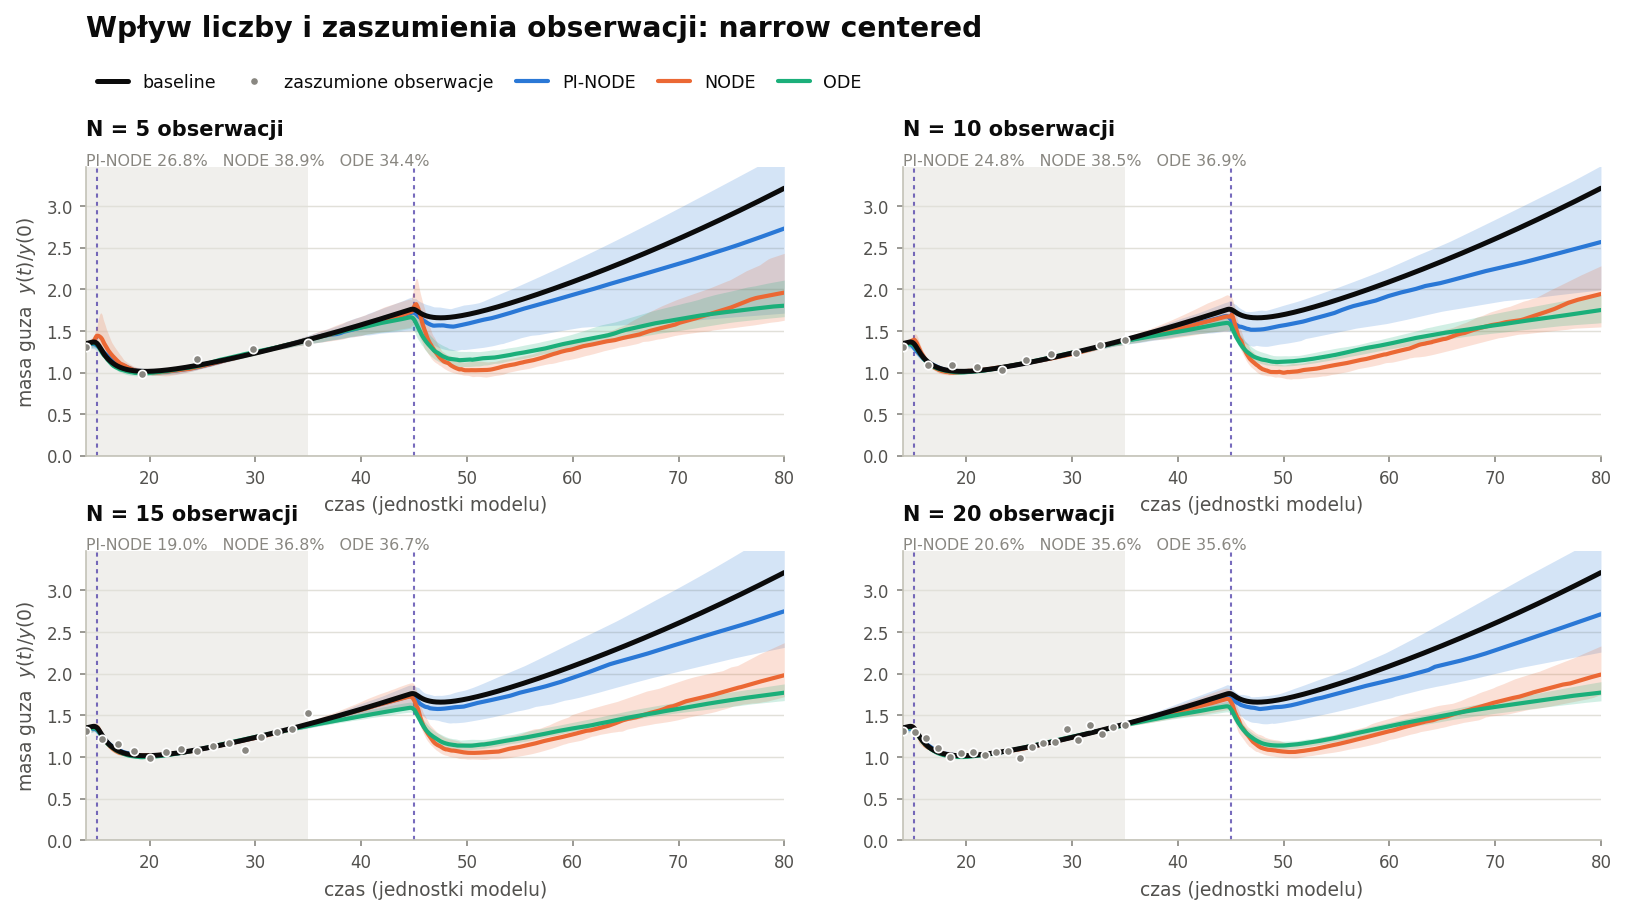
\includegraphics[width=0.95\linewidth]{rys4-pasma-waska-wiazka.png}
\caption{\emph{Narrow centered} jest przypadkiem, w którym redukcja gubi informację.
Mediana PI-NODE (niebieska) dosuwa się do prawdy wraz ze wzrostem $N$ i pasmo się zawęża.}
\label{fig:pasma-waska}
\end{figure}

\begin{table}[H]
\centering\footnotesize
\setlength{\tabcolsep}{5pt}
\begin{tabular}{@{}crrrr@{}}
\toprule
& \multicolumn{2}{c}{\textbf{PI-NODE}} & \multicolumn{2}{c}{\textbf{ODE mechanistyczny}}\\
\cmidrule(lr){2-3}\cmidrule(lr){4-5}
$N$ & obciążenie & szerokość pasma & obciążenie & szerokość pasma\\
\midrule
5  & 21,3\,\% & 6,19 & 40,7\,\% & 0,76\\
10 & \phantom{0}3,9\,\% & 4,72 & 41,4\,\% & 0,71\\
15 & \phantom{0}2,7\,\% & 5,35 & 41,6\,\% & 0,68\\
20 & \phantom{0}9,8\,\% & 3,44 & 40,7\,\% & 0,72\\
\bottomrule
\end{tabular}
\caption{Wąska wiązka, wartości w chwili $t=80$. Obciążenie = odległość mediany zespołu od
prawdy (w \% prawdy); szerokość pasma = rozpiętość percentyli 10--90 w jednostkach masy.}
\label{tab:pasma}
\end{table}

Po przeanalizowaniu Rysunku \ref{fig:pasma-waska} oraz Tabeli \ref{tab:pasma} możemy sformułować poniższe wnioski:

\begin{itemize}
\item \textbf{Model mechanistyczny jest obciążony, a nie niepewny.} Jego obciążenie stoi
na $\approx 41\,\%$ dla \emph{każdego} $N$, a pasmo jest wąskie (0,7). Dokładanie danych
nic nie daje, model jest pewny zwracanego wyniku, bo brakującej
informacji przestrzennej nie da się uzupełnić większą liczbą pomiarów skalarnych.

\item \textbf{PI-NODE jest niepewny, a nie obciążony.} Jego obciążenie spada z 21,3\,\%
przy $N=5$ do 2,7--9,8\,\% od $N=10$ wzwyż, a pasmo zawęża się z 6,19 do 3,44. To błąd
\emph{redukowalny} --- właśnie taki, jaki powinien maleć wraz z jakością danych.

\item \textbf{Od $N=10$ dokładanie próbek daje już niewiele.} Największy skok następuje
między 5 a 10 obserwacjami, dalej zysk jest marginalny. Przy $N=5$ model ma mniej punktów
niż parametrów swobodnych i pasmo nie zbiega.

\item \textbf{Wniosek praktyczny: warto uśredniać po realizacjach szumu.} Mediana zespołu
PI-NODE jest przy $N=15$ oddalona od prawdy o 2,7\,\%, podczas gdy typowe \emph{pojedyncze}
dopasowanie ma błąd 26,5\,\%. Ta różnica jest wyłącznie wariancją, tani zespół
(kilkanaście dopasowań na różnych realizacjach szumu i mediana) powinien zlikwidować
większość tego błędu.
\end{itemize}

\subsection{Ile błędu jest nieusuwalne}

Osobno dopsowałem model mechanistyczny ODE to całej trajektorii, a nie jedynie na przedziale uczącym (na przedziale czasu $[0, 80$). Dzięki temu możliwe jest sprawdzenie, czy model mechanistyczny w ogóle jest w stanie dopasować się do prawdziwych trajektorii. Pozwala to, także oddzielić błąd wynikający z niedopasowania struktury modelu od błędu estymacji. Tabelka \ref{tab:necessary-error} przedstawia uzyskane wyniki.

\begin{table}[H]
\centering\small
\begin{tabular}{@{}lc@{}}
\toprule
\textbf{Wykładnik $q$} & \textbf{Media błędu dopasowania}\\
\midrule
logistyczny ($q=1$)      & 6,96\,\%\\
objętościowy ($q=2/3$)   & 6,79\,\%\\
uczony wykładnik         & 6,24\,\%\\
\bottomrule
\end{tabular}
\caption{Nieusuwalna część błędu przy redukcji dwustanowej.}
\label{tab:necessary-error}
\end{table}

Około 6--7\,\% błędu jest więc nieusuwalne przy tej redukcji, niezależnie od
tego, jak dobrze dopasujemy parametry. Najlepszy nasz model osiąga 11,1\,\%, zatem do
podłogi strukturalnej brakuje około 4 punktów procentowych.

\section{Wagi modeli}
\label{sec:cechowanie}

Funkcja $f_{\mathrm{RT}}$ jest jednorodna stopnia pierwszego względem
$(\rho,\gamma,\mu)$ przy ustalonym $K$. Zatem dla dowolnego $c>0$:
\begin{equation}
\omega\, f_{\mathrm{RT}}(y,z,U;\ \rho,\gamma,K,\mu,\tau)
\;=\;
\frac{\omega}{c}\, f_{\mathrm{RT}}(y,z,U;\ c\rho,\,c\gamma,\,K,\,c\mu,\,\tau).
\label{eq:cechowanie}
\end{equation}

Cokolwiek ustawimy jako $\omega$, optymalizator może to \emph{dokładnie} cofnąć,
przeskalowując $\theta$. To samo dotyczy $s_r$, ponieważ sieć kończy się warstwą afiniczną,
więc $s_r$ wchłania się w jej wagi wyjściowe. To spostrzeżenie sprawdziłem numerycznie. Trajektorie dla $(\omega,\theta)$ i $(\omega/c,\,c\theta)$ oraz odpowiednik dla $s_r$ zgadzają się co do niepewności numerycznej oraz błedów w operacjach zmiennoprzecinkowych.

\subsection{Czy współczynniki można dopasować?}
\label{sec:uczone-wagi}

Aby znaleźć najlepsze parametry $\omega$ i $s_r$, zdecydowałem się przeprowadzić eksperyment, gdzie dopasuje ich wartości razem z zwykłymi parametrami modelu. Niestety to podejście nie ma prawa działać, co możemy wywnioskować z równania~\eqref{eq:cechowanie}. Skoro strata jest dokładnie niezmiennicza wzdłuż kierunku
$(\omega,\theta) \rightarrow (\omega/c,\,c\theta)$, to pochodna wzdłuż tego kierunku wynosi
zero. Gradient nie ma czego minimalizować, więc optymalizator zostaje tam, gdzie go
postawiono (tabela~\ref{tab:uczone-wagi}):

\begin{table}[H]
\centering\footnotesize
\setlength{\tabcolsep}{6pt}
\begin{tabular}{@{}llrrr@{}}
\toprule
\textbf{Start} $(\omega,\,s_r)$ & \textbf{Koniec} $(\omega,\,s_r)$ &
\textbf{Trening} & \textbf{Test} \\
\midrule
$(0{,}005;\,0{,}005)$ & $(0{,}0094;\,0{,}0084)$ & 2,12\,\% & \textbf{15,32\,\%} \\
$(0{,}02;\,0{,}02)$   & $(0{,}0311;\,0{,}0253)$ & 1,88\,\% & 21,01\,\% \\
$(0{,}05;\,0{,}10)$   & $(0{,}0666;\,0{,}1068)$ & 1,77\,\% & 24,86\,\% \\
$(1{,}0;\,1{,}0)$     & $(0{,}8669;\,0{,}9475)$ & 1,88\,\% & \textbf{34,70\,\%} \\
\bottomrule
\end{tabular}
\caption{Wagi uczone razem z resztą modelu. Nie ma śladu
zbieżności do wspólnej wartości.}
\label{tab:uczone-wagi}
\end{table}

Wnioskiem z tego eskperymentu jest konieczność przeprowadznia poszukiwania kombinacji optymalnych wartości parametrów $\omega$ i $s_r$. To przeszukanie zostało zrobione dla kombinacji wartości z przedziału $[0.001, 1] \times [0.001, 1]$. W Tabeli \ref{tab:dokladnosc} zostały użyte wartości parametrów dające najlepsze wyniki. 

\section{Wnioski i dalsze kroki}

Analizując tabele z wynikami, myślę, że jasno możemy stwierdzić, że model PI-NODE ma sens oraz pozwala on na uzyskanie lepszych wyników niż model ODE i NODE w krótkim czasie oraz beż użycia GPU. Wnioski z przeprowadzonych eksperymentów:


\begin{itemize}
\item Redukcja modelu przestrzennego opłaca się ($\approx 350\times$ szybciej, stan
z dwóch liczb zamiast 5,3 mln).

\item PI-NODE bije obie skrajności: 12,76\,\% wobec 29,09\,\% dla samej fizyki
i 32,52\,\% dla samego uczenia.

\item W przypadkach, gdzie redukcja gubi informację przestrzenną, przewaga jest czterokrotna
(7,1\,\% wobec 28,5\,\%), to główna teza projektu i broni się na prawdziwej anatomii.

\item Błąd PI-NODE jest \emph{redukowalny} (wariancja malejąca z liczbą obserwacji),
a błędy obu pozostałych modeli \emph{nie są}: zarówno sama fizyka, jak i sama sieć mają
obciążenie stałe względem $N$, odpowiednio $\approx 45\,\%$ i $\approx 39\,\%$
(rozdz.~\ref{sec:pasma}).

\end{itemize}

Ważne elementy metody:

\begin{itemize}
\item $\omega$ i $s_r$ nie są bilansem ML/Fizyka

\item Nauka współczynników $\omega$ i $s_r$ jest niemożliwa. Kierunek jest płaski, więc wynik zależy
wyłącznie od punktu startowego (rozdz.~\ref{sec:uczone-wagi});

\item $s_r$ można opisać jako jako kontrolę swobody członu uczonego, a nie jako wagę
fizyki, to ona rządzi dokładnością (11,2 punktu wobec 2,6 dla $\omega$). Najmocniej
widać to w zestawieniu PI-NODE z NODE: ta sama sieć, pozbawiona ograniczenia skali,
zachowuje się jak model mechanistyczny, a nie jak model hybrydowy
(rozdz.~\ref{sec:pasma}).
\end{itemize}

Bardzo ważnym wnioskiem jest też znalezienie sufitu dopasowania dla metody dwustanowej względem wartości ground truth. Tabela \ref{tab:necessary-error} pokazuję, że limitem modelu dwustanowego jest relRMSE na poziomie około 6--7 \%, osiągnięcie lepszego wyniku jest po prostu niemożliwe zakładając redukcję.

\end{document}
